
\paragraph{Varicion de la \textit{sparcity}}
Al variar la relaci\'on de cantidad de links frente al tama\~no de la matriz, estamos cambiando que tan rala es la matriz. Para analizar esto,
tomamos en cuenta la \textit{sparcity} la cual representaremos de ahora en m\'as como $\delta = 1 - \frac{n}{m^2}$. A continuaci\'on se muestra 
el gr\'afico obtenido a partir de la experimentiaci\'on dejando fijos $n = 100$, $p = 0.8$, $\varepsilon = 10^{-5}$ y variando $m$ desde $100$
hasta $8000$ de a $100$.

\begin{figure}[h!]
\centering
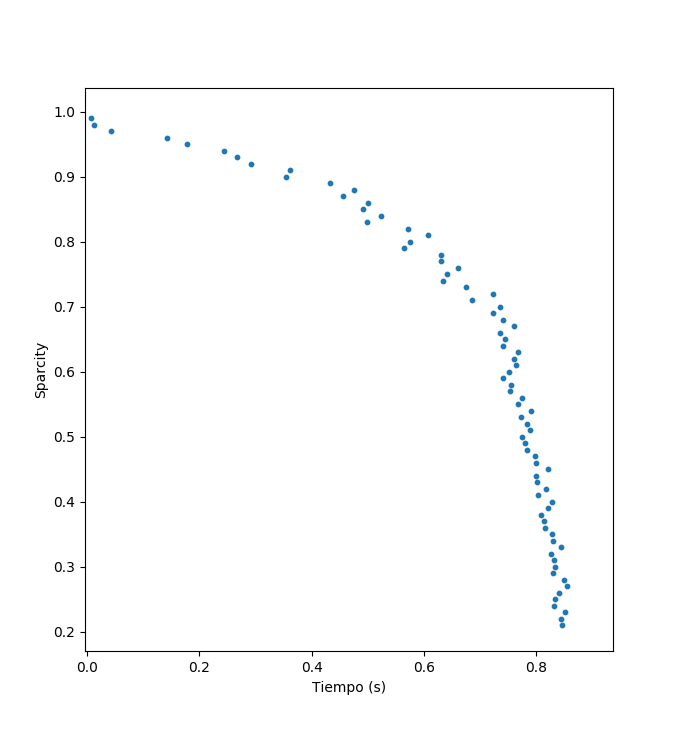
\includegraphics[width=0.7\textwidth]{img/sparcity.png}
\caption{Gr\'afico de sparcity en funci\'on del tiempo}
\label{fig:sparcity}
\end{figure}
A partir de este gr\'afico podemos observar como, tal como fue predicho, que a medida que la matriz es menos rala ($\delta \approx 0$) aumenta
considerablemente el tiempo que demora en ejecutarse el algoritmo.


\paragraph{Varicion de la probabilidad}
Para analizar la incidencia de la probabilidad en el tiempo requerido, tomamos como par\'ametros fijos $n = 1000$, $m$ = 500,
$\varepsilon = 10^{-5}$ y variamos $p$ desde $0.01$ hasta $0.99$ con un incremeto de $0.01$ en cada paso.

\begin{figure}[h!]
\centering
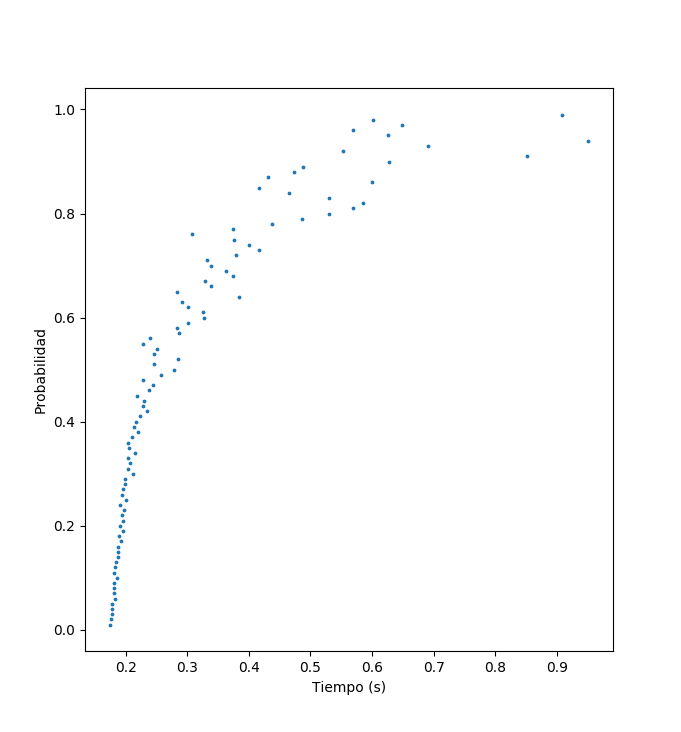
\includegraphics[width=0.7\textwidth]{img/Proba.png}
\caption{Gr\'afico de probabilidad en funci\'on del tiempo}
\label{fig:proba}
\end{figure}

Se puede apreciar como la elecci\'on de la probabilidad tambi\'en afecta en el tiempo de ejecuc\'on, tal como nos im\'aginabamos previo al experimento.

\paragraph{Varicion del epsilon}

Para analizar c\'omo afecta el $\varepsilon$ con el tiempo, tomamos como par\'ametros fijos $n = 1000$, $m$ = 500,
$\varepsilon = 10^{-5}$ y variamos $p$ desde $0.01$ hasta $0.99$ con un incremeto de $0.01$ en cada paso.

\begin{figure}[h!]
\centering
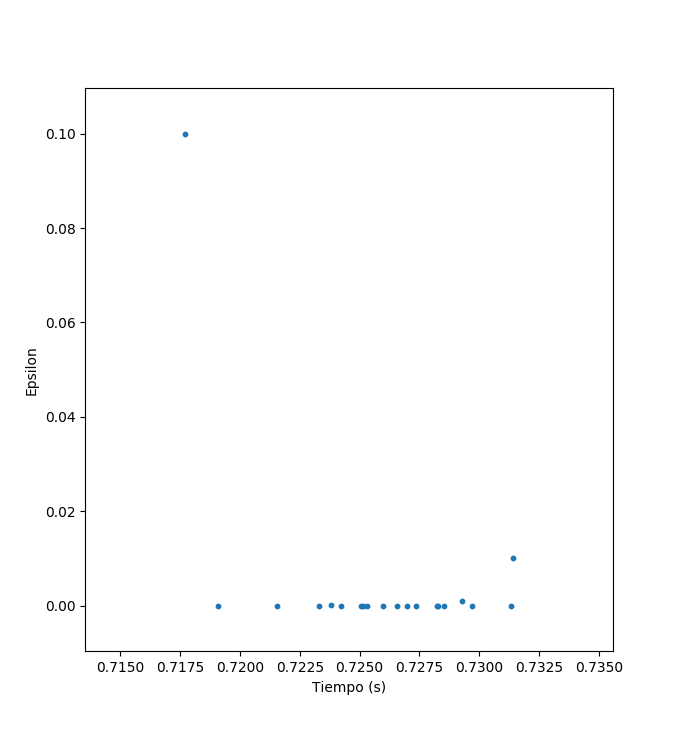
\includegraphics[width=0.7\textwidth]{img/Eps.png}
\caption{Gr\'afico de epsilon en funci\'on del tiempo}
\label{fig:proba}
\end{figure}

Aqui, pese a correr varias veces el test con distintos valores, no logramos apreciar correlaci\'on alguna entre la variaci\'on del $\varepsilon$ y el
tiempo.